\section{Verbesserung der Augen}
\label{verbesserung_ElSe}
Zusätzlich zu den 64 Landmarks, die ein Gesicht beschreiben, kann von OpenFace weitere 28 Landmarks für ein Auge bestimmt werden, aus denen dann die Blickrichtung ermittelt wird.\\
Um die Position der Landmarks zu verbessern, kann auf dem Bildausschnitt der Augen der ElSe-Algotithmus eingesetzt werden. Dieser Algorithmus arbeitet auf einem Farbbild um so die Umrisse der Pupille zu berechnen.\\
Da unter den 28 Landmarks die Umrisse von Pupille und Iris beschreiben wird, müssen diese aus dem Ergebnis von ElSe abgeleitet werden. Dabei hat sich eine Veränderung des Radius mit ?? für Pupille und ?? für die Iris bewährt.\\
Allerdings muss das Auge für die Berechnung aus entsprechend vielen Pixeln bestehen, wodurch es im Originalbild mindestens mit 10 Pixeln dargestellt wird, um sinnvolle Ergebnisse zu erhalten. Da diese Berechnung unabhängig der Landmarks ausgeführt wird, empfiehlt sich das Ergebnis zu überprüfen, damit die bestimmte Ellipse auch innerhalb der Augenhöhle liegt.\\
Dabei wird jedes Auge unabhängig vom anderen betrachtet, wodurch sich verschiedene Blickrichtung ergeben. Ab einer Distanz von mehr als ??cm kann die Blickrichtung beider Augen als parallel angesehen und kann entsprechend behandelt werden. Eine Verbesserung ergibt sich, wenn beide Augen anhängig von einander bestimmt werden, damit sich der Fehler minimiert.
\subsection{Auswirkung der verschiedenen Verfahren}
Um die einzelnen Verfahren besser Vergleichen zu können wurden künstliche Augen aus dem Datensatz \cite{database_Eye} verwendet, da die Exakte Position der Landmarks bekannt sind.
Da auch in der späteren Anwendung der Augenbereich genauer bestimmt ist, bevor ElSe zum Einsatz kommt wurde, nur der Bildbereich in dem alle Landmarks der Augenlider liegen, somit sind die Bilder etwa 64 auf 29 Pixel groß. Um die Qualität der Berechnung bei verschiedenen Größen zu simulieren, wurde das Bild um den angegebenen Faktor linear verkleinert.\\
Ein gutes Verfahren muss stabil gegenüber der Skalierung sein damit es auch auf kleinen Bereichen zuverlässig arbeitet. Da für die spätere Anwendung vor allem das Zentrum der Pupille von Interesse ist, wird der Abstand zum Zentrum als Qualitätsmaß verwendet.\\
\begin{figure}
	\centering
	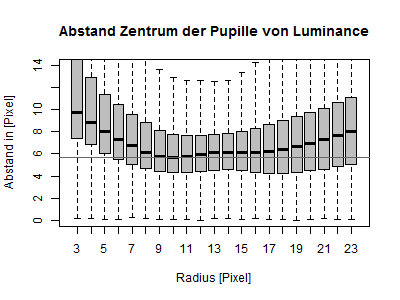
\includegraphics[width=0.32\linewidth]{Eye_Img_Box/Norm_Radius_A}
	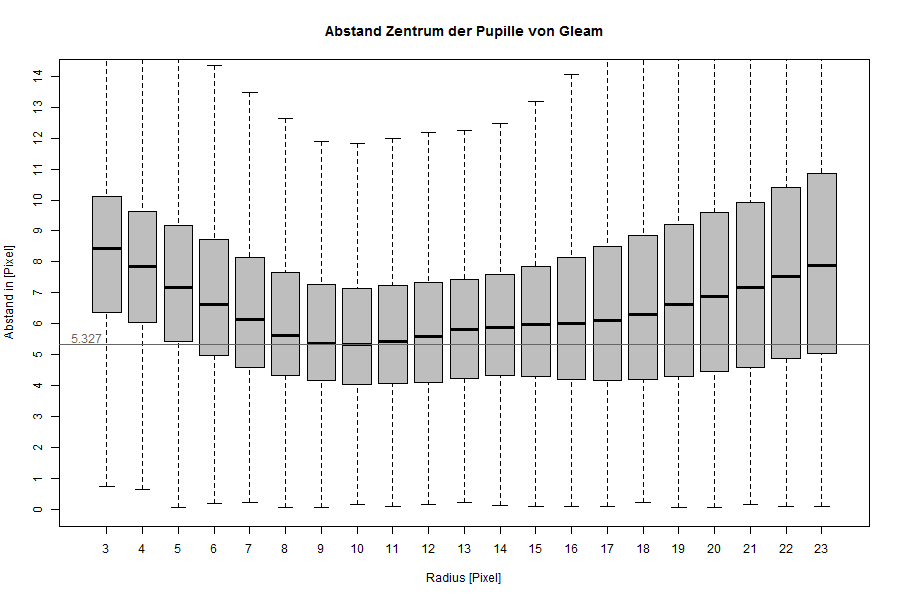
\includegraphics[width=0.32\linewidth]{Eye_Img_Box/Gleam_Radius_A}
	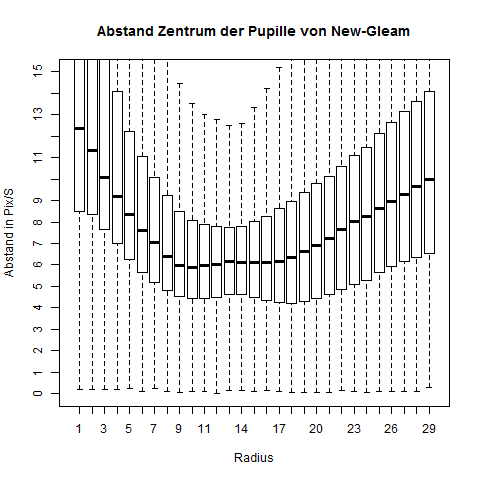
\includegraphics[width=0.32\linewidth]{Eye_Img_Box/New_Radius_A}
	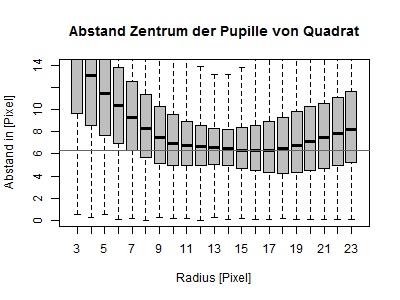
\includegraphics[width=0.32\linewidth]{Eye_Img_Box/Qua_Radius_A}
	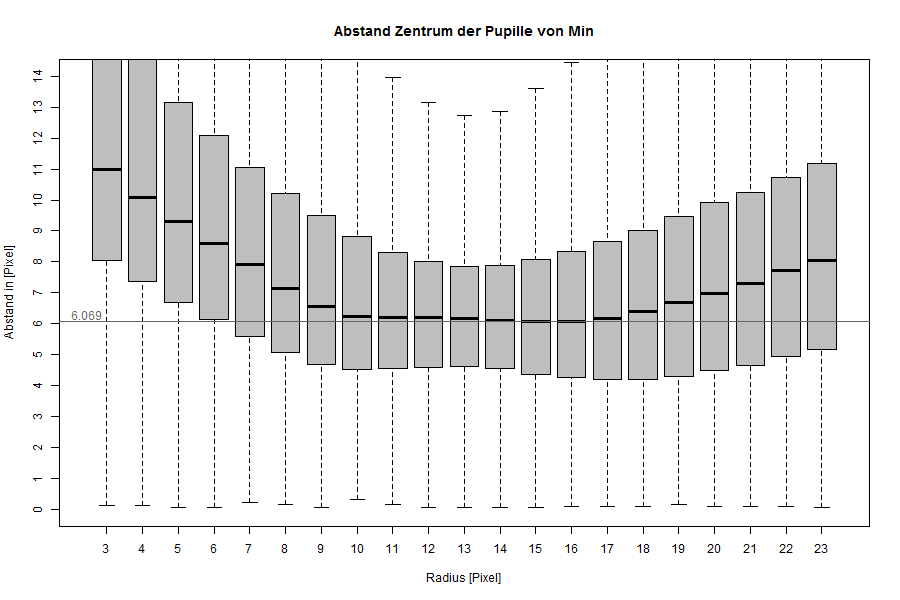
\includegraphics[width=0.32\linewidth]{Eye_Img_Box/Min_Radius_A}
	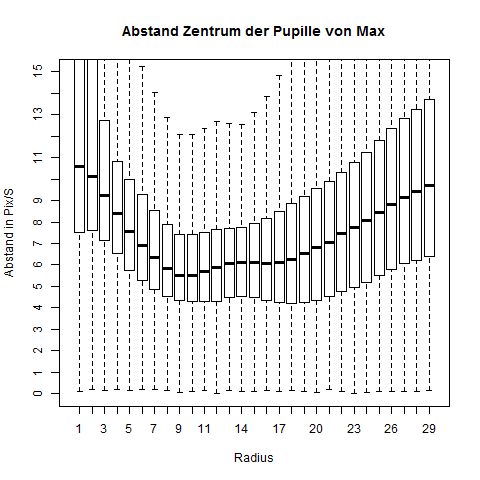
\includegraphics[width=0.32\linewidth]{Eye_Img_Box/Max_Radius_A}
	%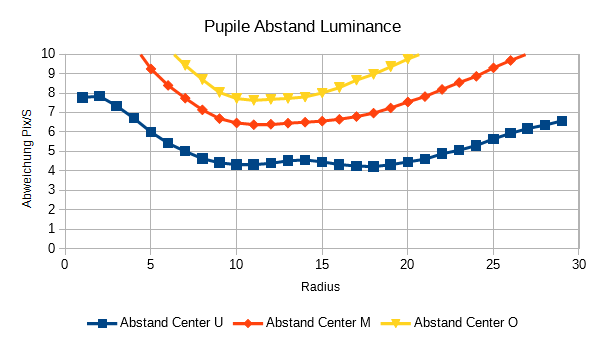
\includegraphics[width=0.49\linewidth]{Eye_Img/Normal_Abstand_P}
	%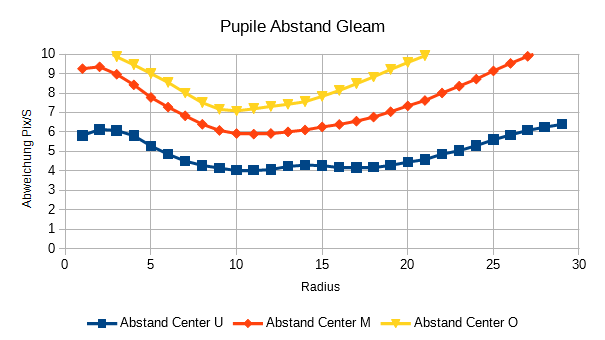
\includegraphics[width=0.49\linewidth]{Eye_Img/Gleam_Abstand_P}
	%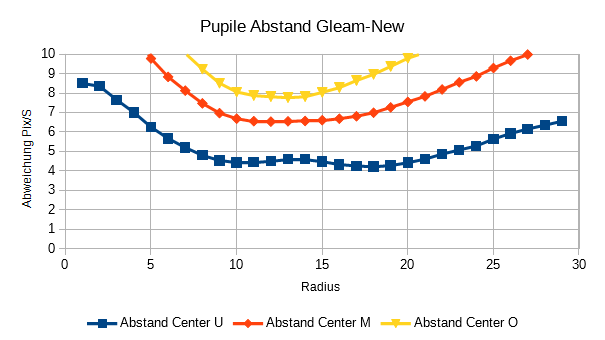
\includegraphics[width=0.49\linewidth]{Eye_Img/New_Abstand_P}
	%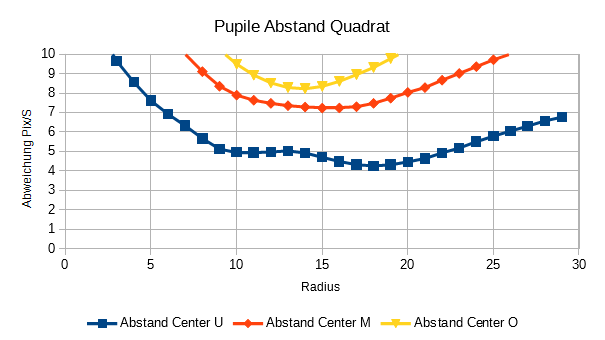
\includegraphics[width=0.49\linewidth]{Eye_Img/Quadrat_Abstand_P}
	%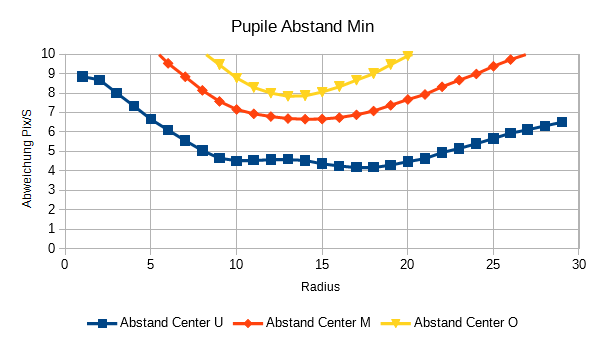
\includegraphics[width=0.49\linewidth]{Eye_Img/Min_Abstand_P}
	%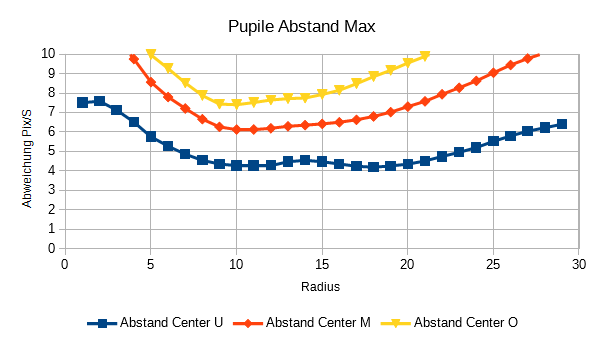
\includegraphics[width=0.49\linewidth]{Eye_Img/Max_Abstand_P}
	\caption{Abstand des Zentrums der Landmark-Pupille und der Berechneten Ellipse in [Pixel/Skalierung]\\Oben-Links: Luminance, Oben-Mitte: Gleam, Oben-Rechts: Gleam New, Unten-Links: Quadrat, Unten-Mitte: Min-Wert, Unten-Rechts: Max-Wert}
	\label{ElSe_Gray_Zentrum}
\end{figure}
\begin{figure}
	\centering
	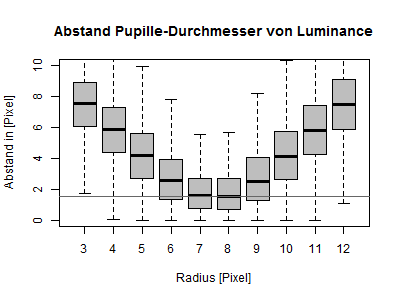
\includegraphics[width=0.32\linewidth]{Eye_Img_Box/Norm_Radius_P}
	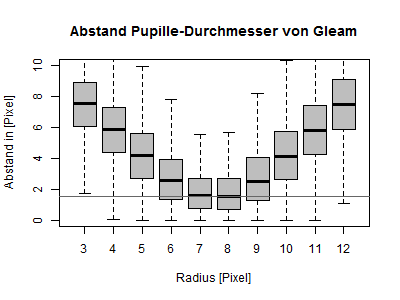
\includegraphics[width=0.32\linewidth]{Eye_Img_Box/Gleam_Radius_P}
	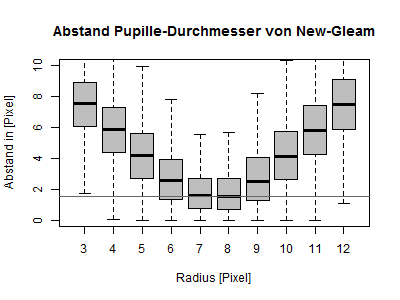
\includegraphics[width=0.32\linewidth]{Eye_Img_Box/New_Radius_P}
	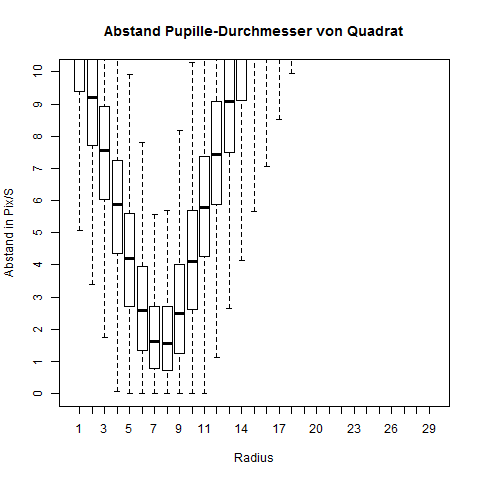
\includegraphics[width=0.32\linewidth]{Eye_Img_Box/Qua_Radius_P}
	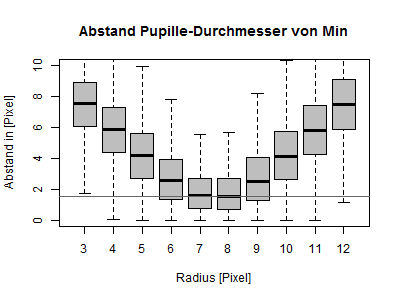
\includegraphics[width=0.32\linewidth]{Eye_Img_Box/Min_Radius_P}
	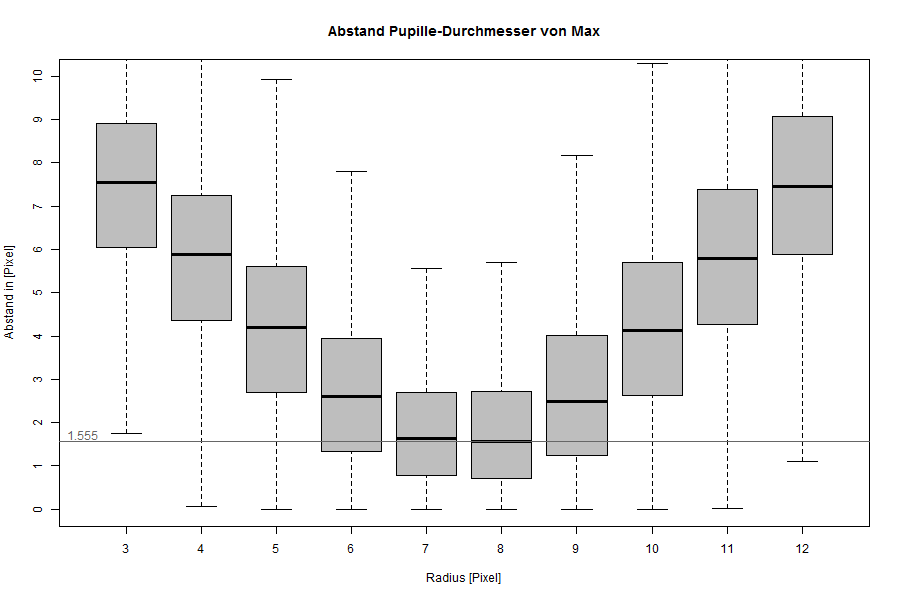
\includegraphics[width=0.32\linewidth]{Eye_Img_Box/Max_Radius_P}
	%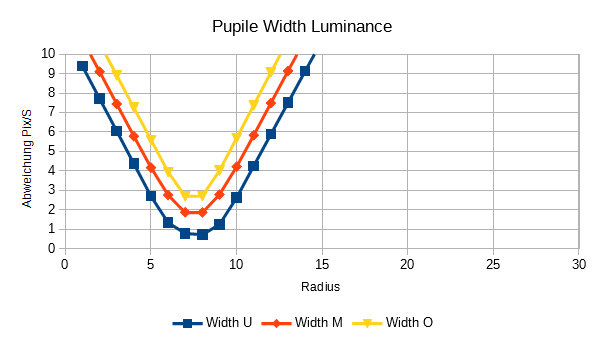
\includegraphics[width=0.49\linewidth]{Eye_Img/Normal_Width_P}
	%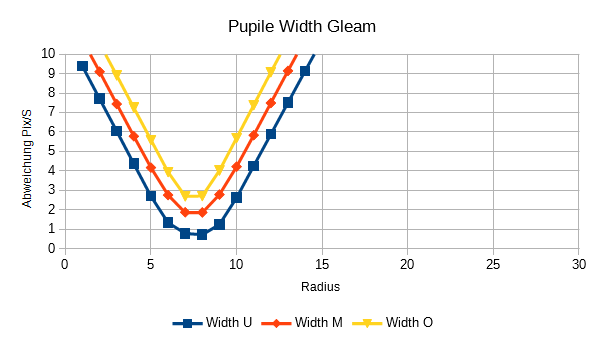
\includegraphics[width=0.49\linewidth]{Eye_Img/Gleam_Width_P}
	%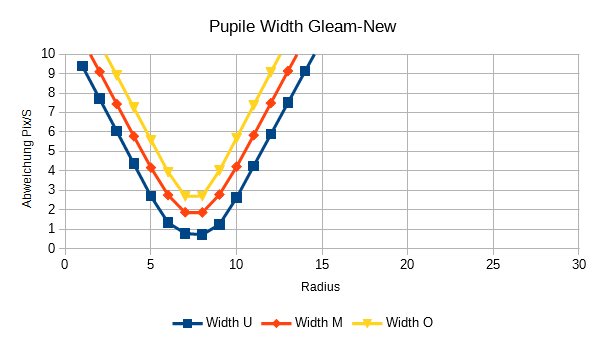
\includegraphics[width=0.49\linewidth]{Eye_Img/New_Width_P}
	%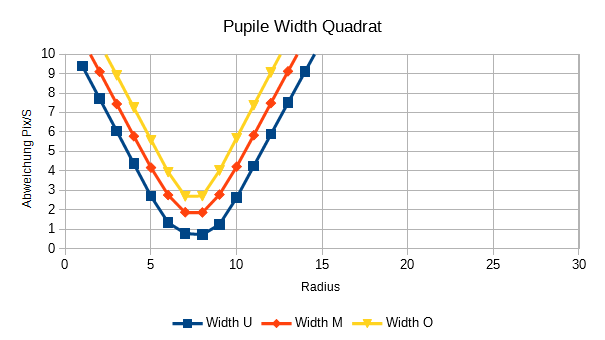
\includegraphics[width=0.49\linewidth]{Eye_Img/Quadrat_Width_P}
	%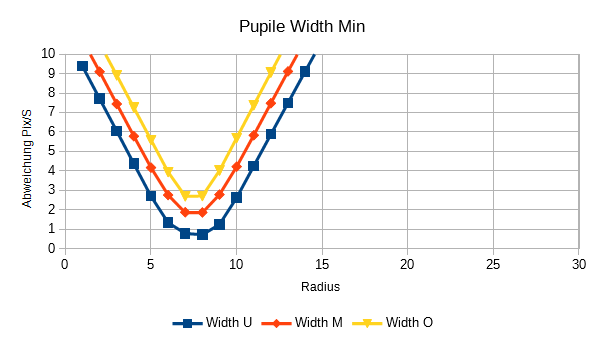
\includegraphics[width=0.49\linewidth]{Eye_Img/Min_Width_P}
	%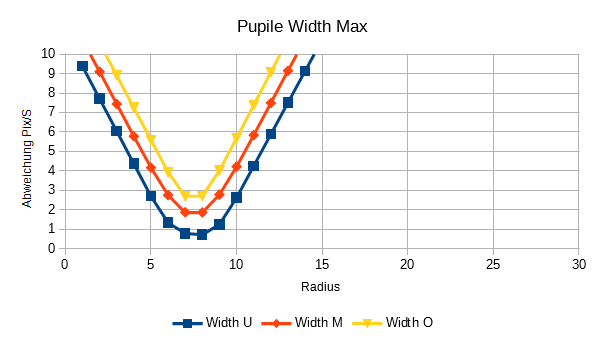
\includegraphics[width=0.49\linewidth]{Eye_Img/Max_Width_P}
	\caption{Unterschied Zwischen den Radien der Landmark-Pupille und der Berechneten Ellipse in [Pixel/Skalierung]\\Oben-Links: Luminance, Oben-Mitte: Gleam, Oben-Rechts: Gleam New, Unten-Links: Quadrat, Unten-Mitte: Min-Wert, Unten-Rechts: Max-Wert}
	\label{ElSe_Gray_Pupille}
\end{figure}
\begin{figure}
	\centering
	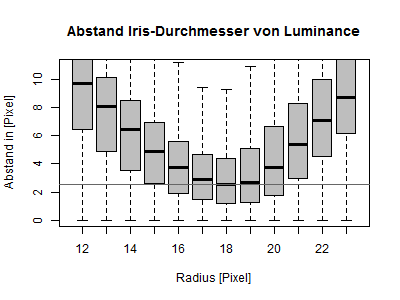
\includegraphics[width=0.32\linewidth]{Eye_Img_Box/Norm_Radius_I}
	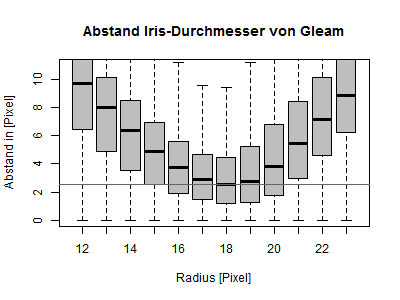
\includegraphics[width=0.32\linewidth]{Eye_Img_Box/Gleam_Radius_I}
	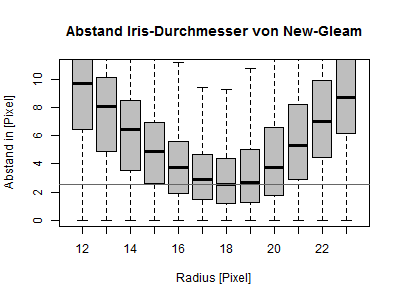
\includegraphics[width=0.32\linewidth]{Eye_Img_Box/New_Radius_I}
	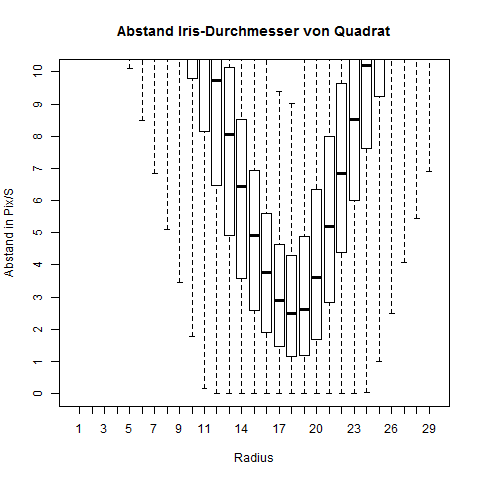
\includegraphics[width=0.32\linewidth]{Eye_Img_Box/Qua_Radius_I}
	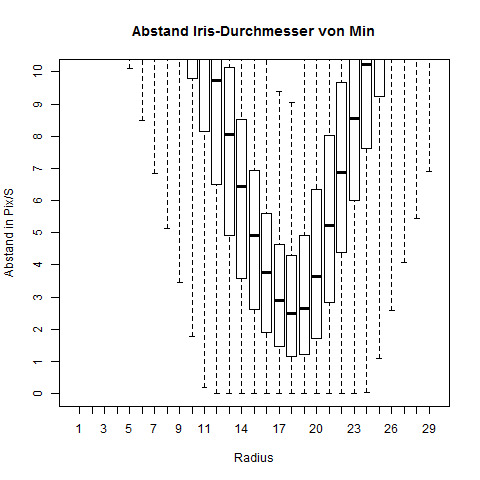
\includegraphics[width=0.32\linewidth]{Eye_Img_Box/Min_Radius_I}
	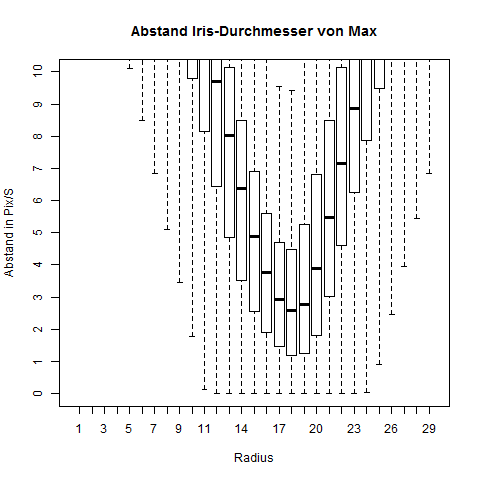
\includegraphics[width=0.32\linewidth]{Eye_Img_Box/Max_Radius_I}
	%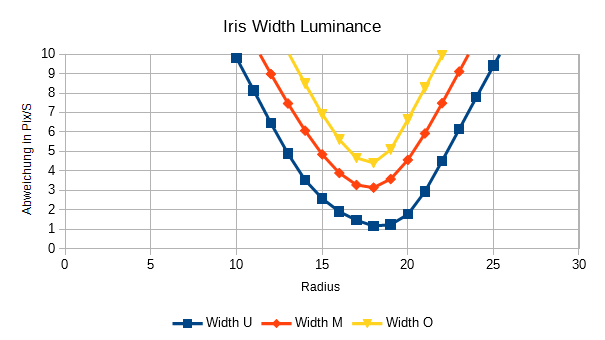
\includegraphics[width=0.49\linewidth]{Eye_Img/Normal_Width_I}
	%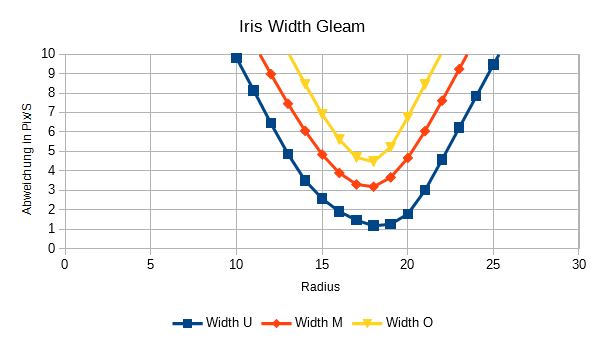
\includegraphics[width=0.49\linewidth]{Eye_Img/Gleam_Width_I}
	%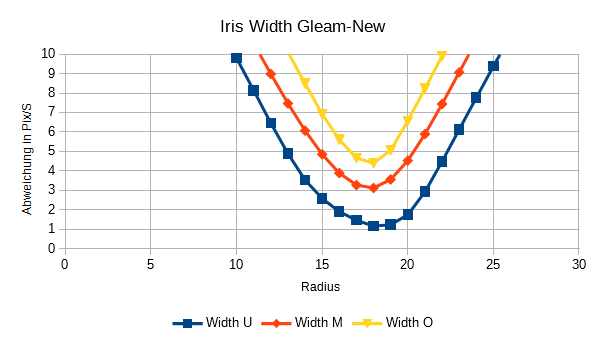
\includegraphics[width=0.49\linewidth]{Eye_Img/New_Width_I}
	%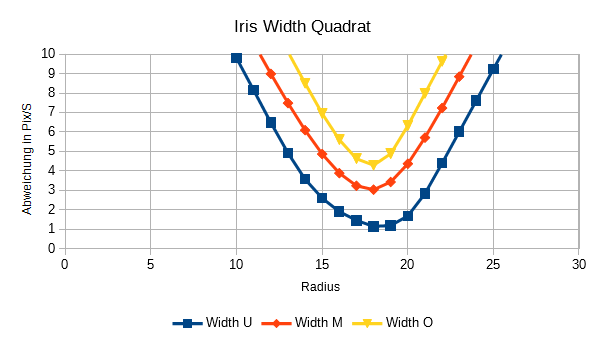
\includegraphics[width=0.49\linewidth]{Eye_Img/Quadrat_Width_I}
	%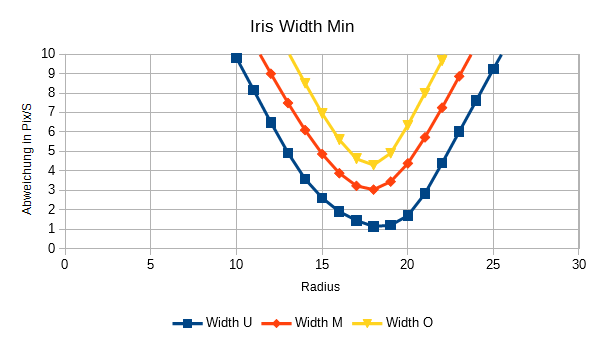
\includegraphics[width=0.49\linewidth]{Eye_Img/Min_Width_I}
	%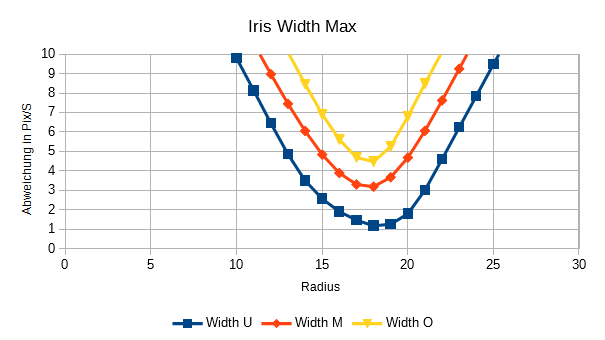
\includegraphics[width=0.49\linewidth]{Eye_Img/Max_Width_I}
	\caption{Unterschied Zwischen den Radien der Landmark-Iris und der Berechneten Ellipse in [Pixel/Skalierung] gegen die Radius-Größe.\\ Oben-Links: Luminance, Oben-Mitte: Gleam, Oben-Rechts: Gleam New, Unten-Links: Quadrat, Unten-Mitte: Min-Wert, Unten-Rechts: Max-Wert}
	\label{ElSe_Gray_Iris}
\end{figure}
Es Zeigt sich, dass das Verfahren um den Farbwert in einen Grauwert zu überführen durchaus Auswirkungen vor allem auf die Positionsbestimmung hat.\\
Als Bestes Verfahren stellte sich Geam heraus, siehe \autoref{ElSe_Gray_Zentrum}, da die Abweichung vom Zentrum minimal ist. Der Unterschied zwischen den einzelnen Verfahren ist signifikant. Ein Mittleres Ergebnis liefert das Luminance-Verfahren, \autoref{gray_Luminance}, mit welchem eine Abweichung auf dem Augen-Trainingsdatensatz \cite{database_Eye} von 6.42 Pixel erreicht wird.\\
Im Vergleich liefert das Quadratische-Verfahren \autoref{gray_Quadrat} im Test die schlechtesten Ergebnis, da die durchschnittliche Abweichung bei 7.23 Pixel liegt. Diese Ungenauigkeit lässt sich wahrscheinlich auf den fehlenden Farbunterschied zwischen Iris und Pupille  zurück zu führen ist.\\
Das beste Ergebnis wurde mit Geam erreicht, eine mittlere Abweichung von 5.89 Pixel. Durch die Gamma-Korrektur ist zwar die Kontur der Iris deutlich schlechter zu detektieren, dies wird allerdings durch die Genauigkeit bei weiten wett gemacht.\\
\begin{figure}
	\centering
	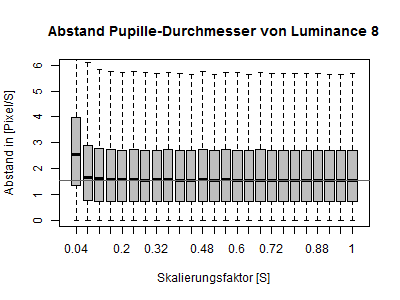
\includegraphics[width=0.32\linewidth]{Eye_Img_Box/Norm_Radius_P_8}
	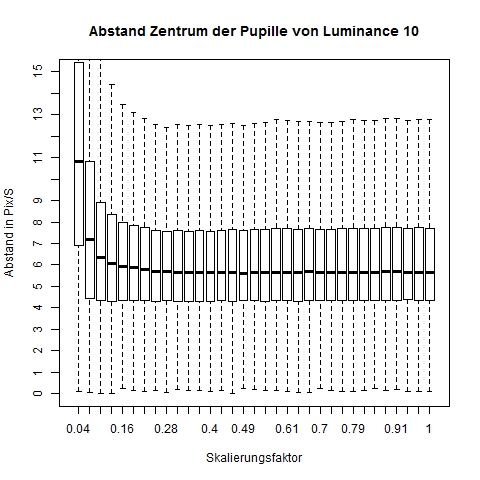
\includegraphics[width=0.32\linewidth]{Eye_Img_Box/Norm_Radius_A_10}
	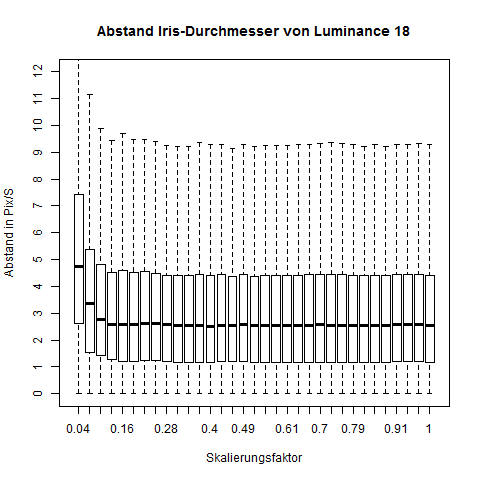
\includegraphics[width=0.32\linewidth]{Eye_Img_Box/Norm_Radius_I_18}\\
	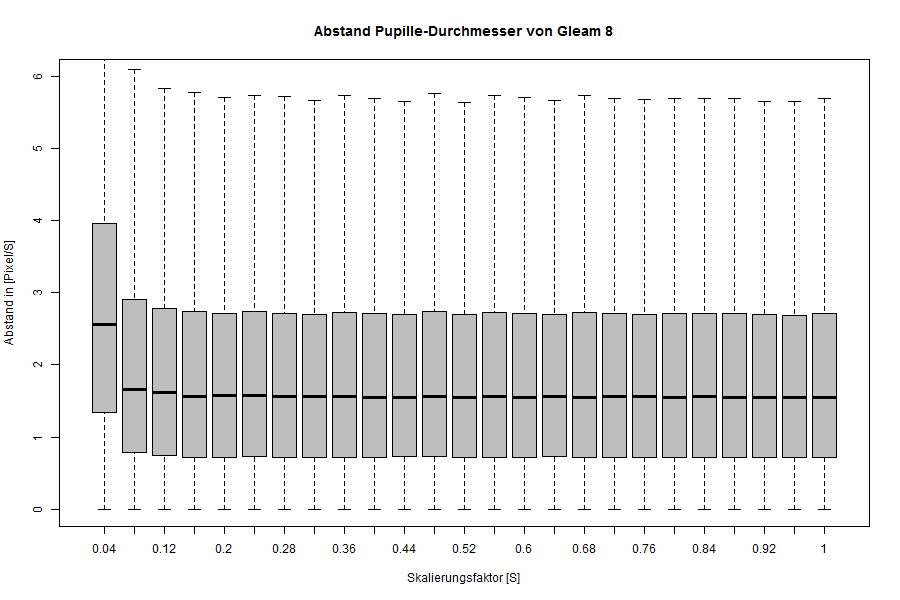
\includegraphics[width=0.32\linewidth]{Eye_Img_Box/Gleam_Radius_P_8}
	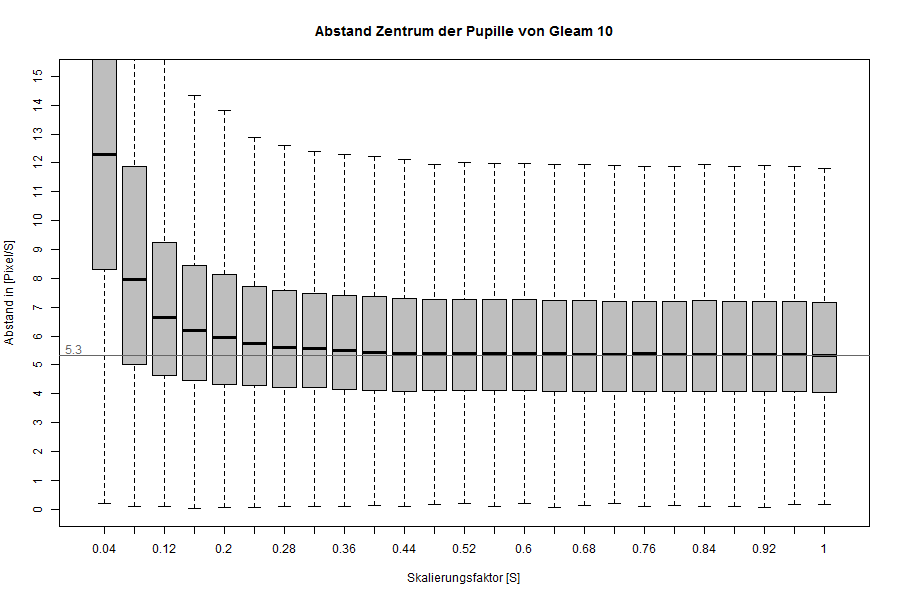
\includegraphics[width=0.32\linewidth]{Eye_Img_Box/Gleam_Radius_A_10}
	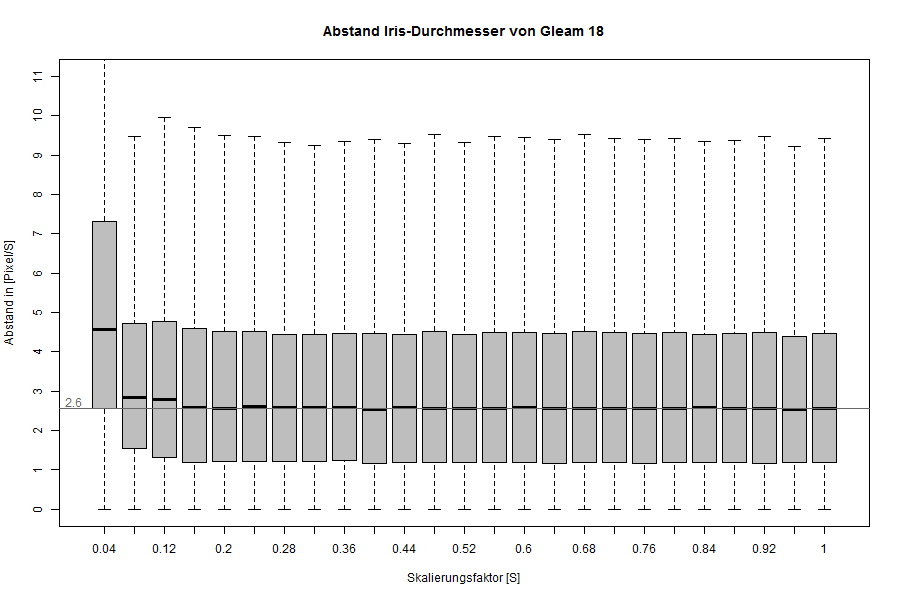
\includegraphics[width=0.32\linewidth]{Eye_Img_Box/Gleam_Radius_I_18}
	%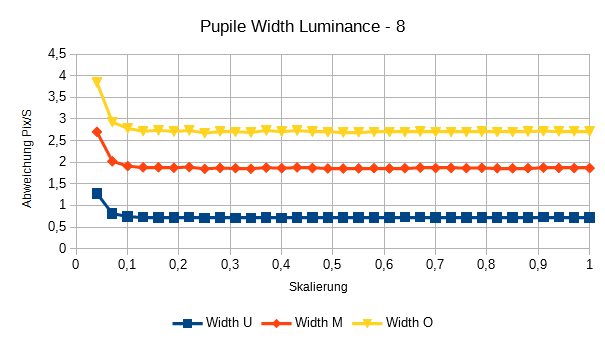
\includegraphics[width=0.32\linewidth]{Eye_Img/Normal_Width_P_8}
	%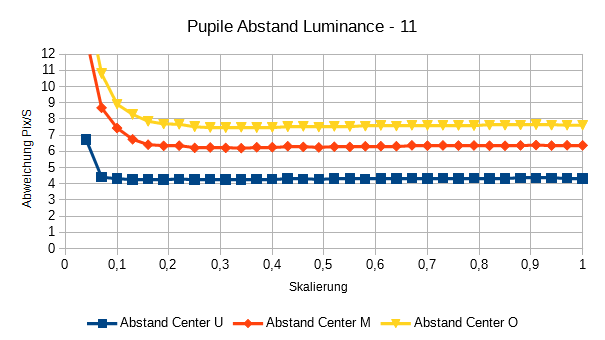
\includegraphics[width=0.32\linewidth]{Eye_Img/Normal_Abstand_P_11}
	%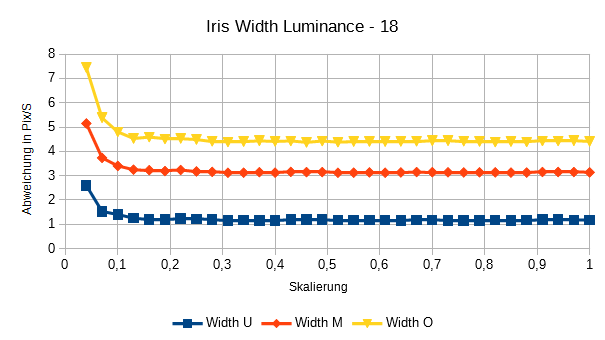
\includegraphics[width=0.32\linewidth]{Eye_Img/Normal_Width_I_18}\\
	%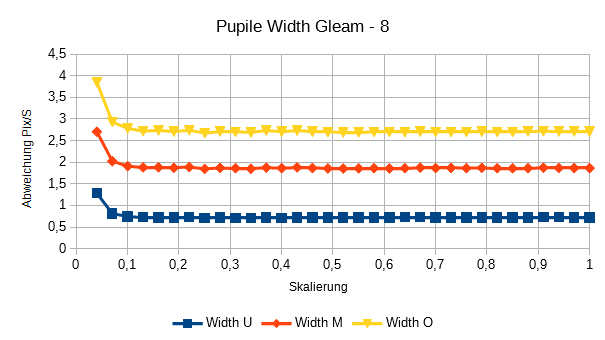
\includegraphics[width=0.32\linewidth]{Eye_Img/Gleam_Width_P_8}
	%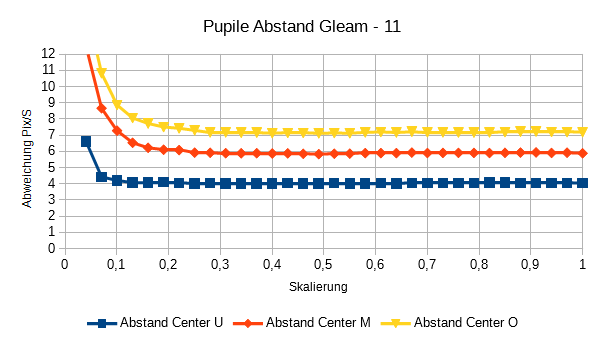
\includegraphics[width=0.32\linewidth]{Eye_Img/Gleam_Abstand_P_11}
	%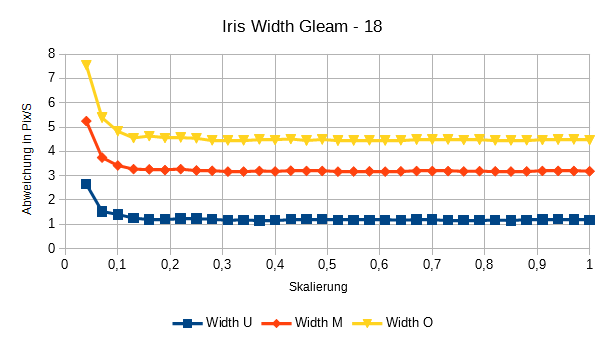
\includegraphics[width=0.32\linewidth]{Eye_Img/Gleam_Width_I_18}
	\caption{Auswirkung von der Bildgröße auf die Qualität der Berechnung.\\ Oben: Luminance, Unten Gleam}
	\label{ElSe_scall}
\end{figure}
Da die Abweichung von ElSe konstant bei etwa 5.9 Pixel bei Glean liegt, arbeitet ElSe stabil bei den Skalierungen, siehe \autoref{ElSe_scall}, womit es vor allem bei kleinen Bildern zuverlässig Ergebnisse liefern kann als OpenFace.\\
So ist im Test der Durchschnitt bei alles Skalierungen ElSe den Ergebnisse von OpenFace überlegen, durch die Verteilung ist allerdings eine Kombination beider Verfahren sinnvoll, so kann das Ergebnis von OpenFace bei Bilder in denen die Iris größer als 21 Pixel ist direkt als Lösung verwendet werden, da der mögliche Fehler von OpenFace geringer ist als von ElSe.\\
Im Bereich zwischen 21 und 15 Pixel können beide Ergebnisse Kombiniert werden, beide Verfahren arbeiten ungefähr gleich gut. Sollte die Iris im Originalbild noch kleiner sein, so ist auf ElSe mehr verlass, da es noch bis zu einer Irisgröße von 3 Pixel noch stabil funktioniert.
\subsection{ElSe - Auswirkung des Radius}
Ein weiter wichtiger Parameter des ElSe-Verfahrens ist der Radius des Filters. Wiederrum wurde der Augen-Datensatz \cite{database_Eye} verwendet und das Auge ausgeschnitten um diesen Bereich auf 384 Pixel als Eingabebild für ElSe zu vergrößern. Im Datensatz besitzen die abgebildeten Augen eine Durchschnittlich Pupille von 15 Pixel und eine Iris von 34 Pixel.\\
In \autoref{ElSe_Gray_Iris} und \autoref{ElSe_Gray_Zentrum} ist zu erkennen, dass die Wahl des Radius signifikant für die Qualität der Berechnung ist. Da für die spätere Anwendung vor allem das Zentrum der Pupille von Interesse ist, siehe \autoref{OpenFace_Blickrichtung}, muss ElSe in diesem Aspekt zuverlässige Ergebnisse liefern.\\
Im Versuch hat sich ein Radius von etwa einem Zwölftel des zu erwartetem Durchmesser der Iris bzw. Pupille als sinnvoll erwiesen, siehe \autoref{ElSe_Gray_Zentrum} und \autoref{ElSe_Gray_Pupille} um deren Dimension möglichst exakt zu bestimmen. Im Versuch entspricht dies 8 und 18 Pixel. Um die Position des Zentrums  der Iris und der Pupille möglichst gut zu bestimmen, erwies sich ein Radius von 11 am besten, siehe \autoref{ElSe_Gray_Zentrum}, wobei der Fehler nicht so sehr steigt bei Veränderung des Radius, als bei der Größenbestimmung von Pupille und Iris.
\subsection{OpenFace}
Als Referenz wird das Ergebnis von OpenFace für die zusätzlich bestimmten Landmarks der Augen verwendet. Dies wurde auch auf dem Augendatensatz \cite{database_Eye} angewendet um vergleichbare Ergebnisse zu erhalten.\\
\begin{figure}
	\centering
	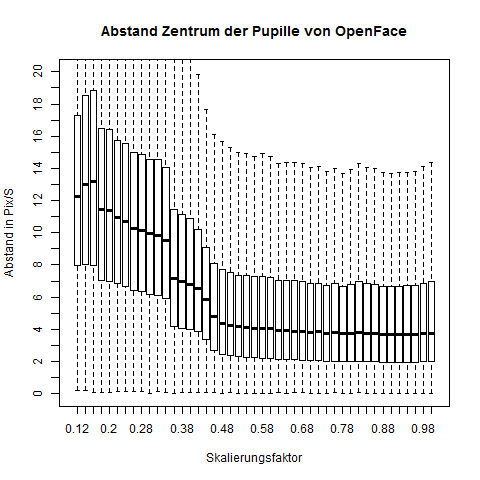
\includegraphics[width=0.45\linewidth]{Eye_Img_Box/Openface_PC}
	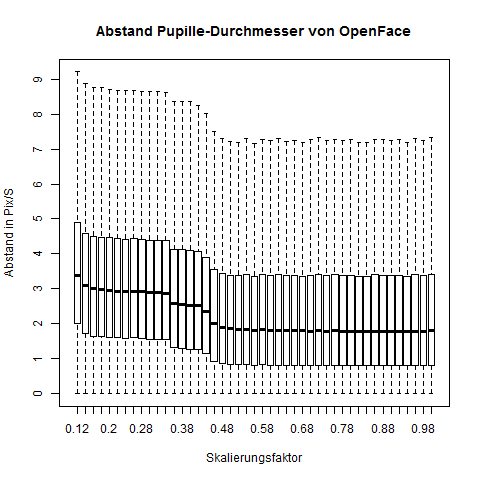
\includegraphics[width=0.45\linewidth]{Eye_Img_Box/Openface_PW}
	%\includegraphics[width=0.45\linewidth]{Eye_Img/OpenFace_Zentrum_P}
	%\includegraphics[width=0.45\linewidth]{Eye_Img/OpenFace_Width_P}
	\caption{Auswirkung von Skalierung auf die Qualität der Augendetektion von ObenFace}
	\label{OpenFace_Eye}
\end{figure}
Es ist zu erkennen dass dieses Verfahren im Schnitt oft schlechtere Ergebnisse liefert als das Ergebnis von ElSe, allerdings ohne das begehen von großen Fehlern und auch öfters genauere Ergebnisse.\\
Da die hohe Qualität von ElSe nur erreicht werden kann, wenn es auf den passenden Bildausschnitt angewendet wird, ist auch die Detektion des Auge von Interesse.\\
\begin{figure}
	\centering
	\includegraphics[width=0.245\linewidth]{Eye_Img_Box/Openface_BoxX}
	\includegraphics[width=0.245\linewidth]{Eye_Img_Box/Openface_BoxY}
	\includegraphics[width=0.245\linewidth]{Eye_Img_Box/Openface_BoxW}
	\includegraphics[width=0.245\linewidth]{Eye_Img_Box/Openface_BoxH}
	%\includegraphics[width=0.245\linewidth]{Eye_Img/Box_X}
	%\includegraphics[width=0.245\linewidth]{Eye_Img/Box_Y}
	%\includegraphics[width=0.245\linewidth]{Eye_Img/Box_W}
	%\includegraphics[width=0.245\linewidth]{Eye_Img/Box_H}
	\caption{Bestimmung der Box ums Auge}
	\label{OpenFace_Eye_Box}
\end{figure}
Nach \autoref{OpenFace_Eye_Box} wird der Bereich des Auges zwar nicht so exakt bestimmt, allerdings überdeckt er den relevanten Bereich. Dargestellt sind Koordinaten, X- und Y-Position in Pixel sowie die Ausdehnung, Width und Hight bestenfalls in Pixel relativ zur umschließenden Box der Landmarks. Somit liegen die Landmarks im Bildausschnitt, wodurch er verwendet werden kann als Eingabe von ElSe.\\
